\documentclass{standalone}
\usepackage{tikz}
\usetikzlibrary{positioning, shapes.geometric, calc}

\begin{document}

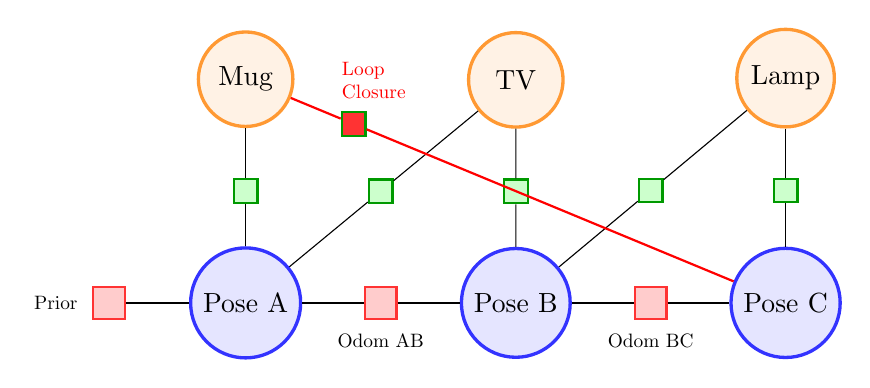
\begin{tikzpicture}[
  node distance=1.5cm and 2cm,
  % Variable Nodes (Circles)
  pose/.style={circle, draw=blue!80, fill=blue!10, very thick, minimum size=1.2cm},
  landmark/.style={circle, draw=orange!80, fill=orange!10, very thick, minimum size=1.2cm},
  % Factor Nodes (Squares)
  motionFactor/.style={rectangle, draw=red!80, fill=red!20, thick, minimum size=0.4cm},
  visionFactor/.style={rectangle, draw=green!60!black, fill=green!20, thick, minimum size=0.3cm}
  ]

  % --- Variable Nodes (States) ---
  \node[pose] (PA) {Pose A};
  \node[pose, right=of PA] (PB) {Pose B};
  \node[pose, right=of PB] (PC) {Pose C};

  \node[landmark, above=of PA] (LMug) {Mug};
  \node[landmark, above=of PB] (LTV)  {TV};
  \node[landmark, above=of PC] (LLamp) {Lamp};

  % --- Motion Factors (The "Odometry" Springs) ---
  \node[motionFactor, left=0.8cm of PA] (FPrior) {};
  \node[left=0.1cm of FPrior, scale=0.7] {Prior};
  
  \node[motionFactor] (FAB) at ($(PA)!0.5!(PB)$) {};
  \node[below=0.1cm of FAB, scale=0.7] {Odom AB};
  
  \node[motionFactor] (FBC) at ($(PB)!0.5!(PC)$) {};
  \node[below=0.1cm of FBC, scale=0.7] {Odom BC};

  % Wiring Motion
  \draw[thick] (FPrior) -- (PA);
  \draw[thick] (PA) -- (FAB) -- (PB);
  \draw[thick] (PB) -- (FBC) -- (PC);

  % --- Vision Factors (The "Measurement" Springs) ---
  % Pose A sees Mug and TV
  \node[visionFactor] (fAM) at ($(PA)!0.5!(LMug)$) {};
  \node[visionFactor] (fAT) at ($(PA)!0.5!(LTV)$) {};
  \draw (PA) -- (fAM) -- (LMug);
  \draw (PA) -- (fAT) -- (LTV);

  % Pose B sees TV and Lamp
  \node[visionFactor] (fBT) at ($(PB)!0.5!(LTV)$) {};
  \node[visionFactor] (fBL) at ($(PB)!0.5!(LLamp)$) {};
  \draw (PB) -- (fBT) -- (LTV);
  \draw (PB) -- (fBL) -- (LLamp);

  % Pose C sees Lamp and Mug (Loop Closure)
  \node[visionFactor] (fCL) at ($(PC)!0.5!(LLamp)$) {};
  \node[visionFactor, fill=red!80] (fCM) at ($(PC)!0.8!(LMug)$) {};
  
  \draw (PC) -- (fCL) -- (LLamp);
  \draw[red, thick] (PC) -- (fCM) -- (LMug);
  \node[red, above left=0.1cm of fCM, anchor=south west, scale=0.7, align=left]
  {Loop \\ Closure};

\end{tikzpicture}

\end{document}
